\begin{figure}[h!]
\centering
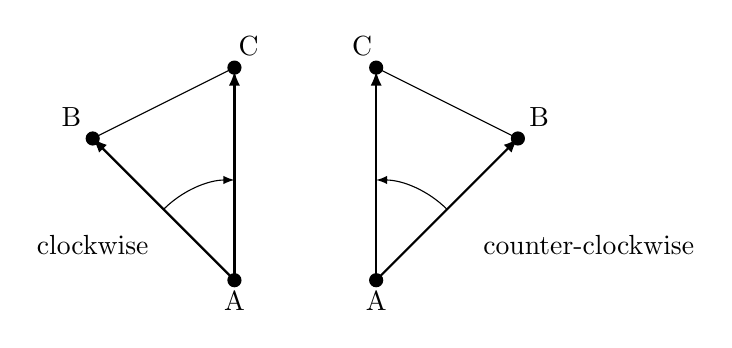
\begin{tikzpicture}[scale=0.9]
\draw[thick, -latex] (2, 0) -- (0,2);
\draw[thick, -latex] (2, 0) -- (2,2.95);
\draw (0,2) -- (2,3);
\fill[black] (2,0) circle (0.1);
\fill[black] (0,2) circle (0.1);
\fill[black] (2,3) circle (0.1);
\draw[-latex] (1,1) arc (135:90:1.4142);
\draw (2,-0.3) node{A};
\draw ((-0.3,2.3) node{B};
\draw (2.2,3.3) node{C};
\draw(0, 0.5) node{clockwise};
\draw[thick, -latex] (4, 0) -- (6,2);
\draw[thick, -latex] (4, 0) -- (4,2.95);
\draw (6,2) -- (4,3);
\fill[black] (4,0) circle (0.1);
\fill[black] (6,2) circle (0.1);
\fill[black] (4,3) circle (0.1);
\draw[-latex] (5,1) arc (45:90:1.4142);
\draw (4,-0.3) node{A};
\draw (3.8,3.3) node{C};
\draw(6.3,2.3) node{B};
\draw(7, 0.5) node{counter-clockwise};
\end{tikzpicture}
\caption{Relative orientation of three points or turning direction of consecutive line segments}
\label{relative}
\end{figure}